% This is part of Un soupçon de mathématique sans être agressif pour autant
% Copyright (c) 2015
%   Laurent Claessens
% See the file fdl-1.3.txt for copying conditions.

\begin{exercice}[\cite{NRHooXFvgpp4}]\label{exo2smath-0149}

    \begin{multicols}{2}

    Sophie qui mesure \SI{1.75}{\meter} est à \SI{30}{\meter} d'un arbre. L'angle entre l'horizontale et le sommet de l'arbre est de \SI{35}{\degree}. Quelle est la hauteur de l'arbre ?

    \columnbreak

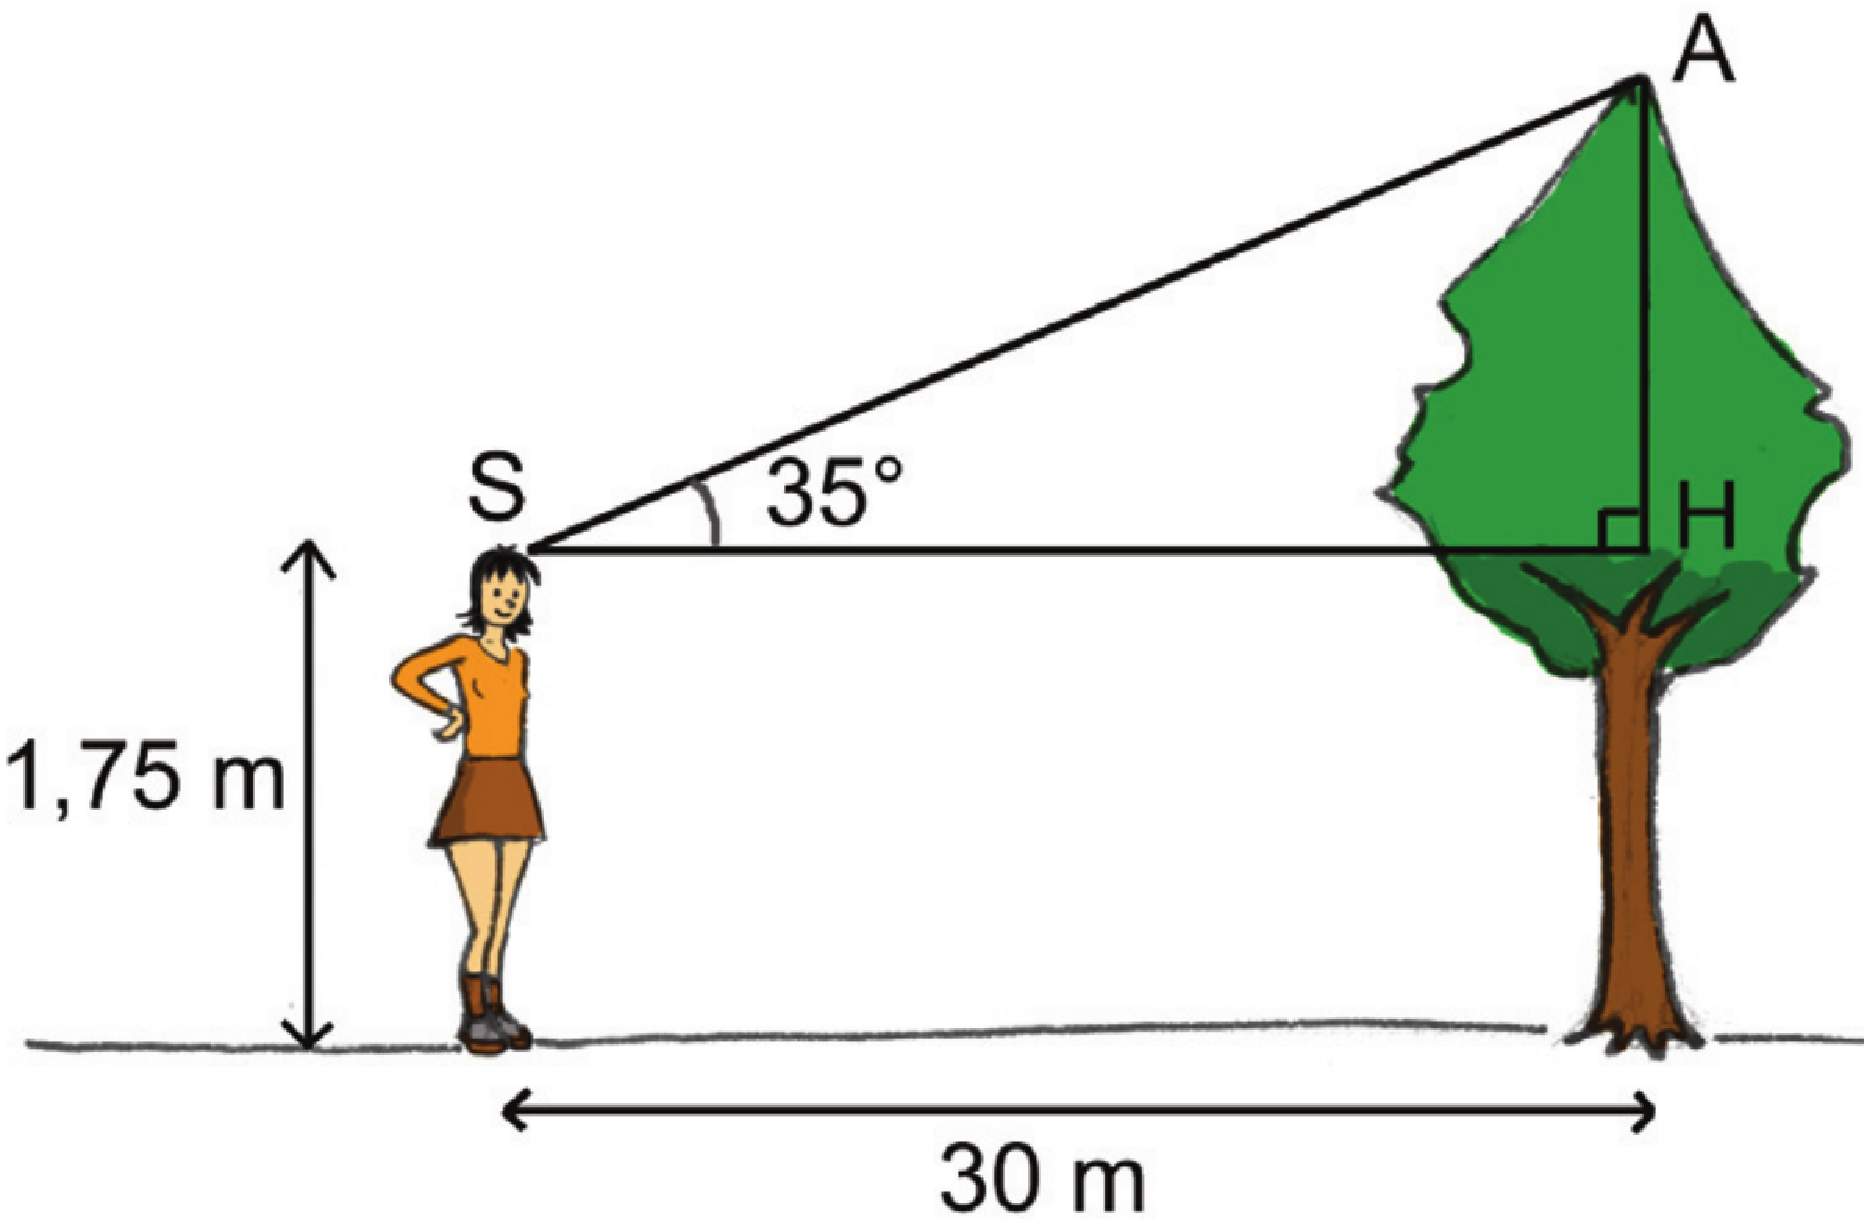
\includegraphics[width=\linewidth]{arbrecosinus.pdf}

    \end{multicols}

\corrref{2smath-0149}
\end{exercice}
